% =============================================================
% Experiment 4
% RC-Coupled Amplifier using BJT in CE Configuration --
% Measurement of Gain, Bandwidth, and Frequency Response
%
% Required packages in the master document preamble:
%   amsmath, amssymb, graphicx, circuitikz, pgfplots, booktabs,
%   enumitem, siunitx, hyperref
%   \pgfplotsset{compat=1.17}
% =============================================================

\chapter{RC-Coupled CE Amplifier using BJT}
\label{chap:expt2}

\section{Aim}
To design, assemble, and test a single-stage RC-coupled amplifier using a BJT in Common-Emitter (CE) configuration. The specific objectives are:
\begin{enumerate}
	\item To verify the DC operating point (Q-point) of the transistor.
	\item To measure the mid-band voltage gain.
	\item To plot its frequency response curve (Gain in dB vs Frequency) on a semi-logarithmic scale.
	\item To determine the lower cutoff frequency ($f_L$), upper cutoff frequency ($f_H$), and overall bandwidth ($BW$).
\end{enumerate}  

\section{Pre-Lab Assignment}
\begin{enumerate}[label=(\roman*)]
	\item Given the supply voltage $V_{CC}$, desired quiescent collector current $I_C$, and BJT parameters ($\beta$, $V_{BE(on)}$) assigned to your batch, design the voltage-divider bias network and calculate $R_1$, $R_2$, $R_C$, $R_E$ for a stable operating point.
	\item Calculate the expected mid-band voltage gain $A_{v(mid)}$ using the design values.
	\item Simulate the designed circuit in LTspice (Pre-Lab~2): run a \texttt{.ac} analysis and obtain the Bode plot (magnitude in dB and phase vs. frequency). Note the lower cutoff frequency $f_L$, upper cutoff frequency $f_H$, and bandwidth $BW = f_H - f_L$ from the simulated plot.
	\item Tabulate the theoretically designed values and the LTspice-simulated values for comparison with hardware measurements to be taken in this experiment.
\end{enumerate}

\section{Components and Equipment Required}
Table~\ref{tab:CompsBJTAmp} lists the components/equipment required.
\begin{table}[htbp!]
	\centering
	\begin{tabular}{@{}cll@{}}
		\toprule
		S.No. & Component/Equipment & Specification \\
		\midrule
		1  & NPN Transistor & BC547 (or equivalent, e.g. BC107), 1 no. \\
		2  & Resistors & $R_1, R_2, R_C, R_E$ as per design \\
		3  & Coupling Capacitors & $C_{in}, C_{out}$ as per design \\
		4  & Bypass Capacitor & $C_E$ as per design \\
		5  & Regulated DC Power Supply & 0--15\,V \\
		6  & Digital Multi-Meter & 0--20\,V\\
		7  & Function Generator & Sine wave, 1\,Hz -- 1\,MHz \\
		8  & Digital Storage Oscilloscope & 2-channel, 20--50\,MHz bandwidth \\
		9  & Breadboard and connecting wires & -- \\
		\bottomrule
	\end{tabular}
	\caption{Components and equipment list for RC-coupled BJT amplifier}
	\label{tab:CompsBJTAmp}
\end{table}
%\clearpage
\section{Theory}
A common-emitter (CE) configuration is widely used in voltage amplification due to its high voltage and current gain, along with moderate input and output impedances. In an RC-coupled amplifier, multiple single-stage amplifiers can be cascaded using a coupling capacitor, though this experiment focuses on analyzing a single-stage implementation. The capacitors $C_{in}$ and $C_{out}$ couple the AC signal into and out of the stage while blocking DC, isolating the amplifier's bias point from the source and the load; an emitter bypass capacitor $C_E$ provides an AC ground at the emitter to maximise gain, while a DC bias network ($R_1, R_2, R_E$) fixes a stable quiescent operating point independent of transistor-to-transistor $\beta$ variation.

\subsection{Circuit Functionality}
\begin{itemize}
	\item \textbf{Biasing Network ($R_1, R_2, R_C, R_E$):} Voltage-divider biasing ($R_1$ and $R_2$) is utilized to provide a stable operating point ($Q$-point) independent of temperature variations and transistor parameter ($\beta$) spreads. $R_C$ serves as the collector load resistor across which the amplified AC output is developed. $R_E$ provides negative feedback to stabilize the DC operating point.
	\item \textbf{Coupling Capacitors ($C_{in}, C_{out}$):} $C_{in}$ blocks any DC component from the AC signal source, preventing it from altering the $Q$-point. Similarly, $C_{out}$ couples the amplified AC signal to the load while blocking the DC voltage at the collector.
	\item \textbf{Bypass Capacitor ($C_E$):} $C_E$ is placed in parallel with $R_E$ to provide a low-impedance path for the AC signal to ground. This prevents AC degeneration across $R_E$, maximizing the mid-band voltage gain.
\end{itemize}
%\subsection{DC Bias Design (Voltage-Divider Bias)}
%The requirements of the bias circuit are:
%\begin{enumerate}
%	\item Keep the B-E junction forward-biased at $\approx 0.7\ \text{V}$.
%	\item Keep the DC operating-point (Q-point) near the middle of the output characteristics, within the operating boundary of $V_{CE}$ and $I_C$. The operating-point is: $\left(I_{CQ},\ V_{CEQ}\right)$.
%\end{enumerate}
%For the potential-divider bias network, assuming the divider current $I_2 \gg I_B$ (typically $I_2 \approx 10\,I_B$), the base voltage is
%\begin{equation}
%	V_B \approx \frac{R_2}{R_1+R_2}\,V_{CC}\,, \qquad V_E = V_B - V_{BE(on)}\,, \qquad I_E \approx I_C = \frac{V_E}{R_E}\,.
%	\label{eq:bias}
%\end{equation}
%The collector resistor $R_C$ is chosen to set the quiescent collector voltage $V_{CQ}$ approximately midway between $V_{CC}$ and $V_E$, so as to allow maximum symmetrical output voltage swing:
%\begin{equation}
%	V_{CQ} \approx \frac{V_{CC}+V_E}{2}\,, \qquad R_C = \frac{V_{CC}-V_{CQ}}{I_C}\,.
%	\label{eq:rc_design}
%\end{equation}

\subsection{Frequency Response Characteristics}
The performance of the amplifier over a wide frequency spectrum is characterized by three distinct bands:
\begin{enumerate}
	\item \textbf{Low-Frequency Region:} At low frequencies, the capacitive reactances of $C_{in}, C_{out},$ and $C_E$ (given by $X_C = 1 / (2\pi fC)$) become significantly high. These reactances drop a considerable portion of the AC signal, thereby reducing the effective voltage gain.
	
	\item \textbf{Mid-Band Region:} In this region (typically \SI{100}{\hertz} to \SI{100}{\kilo\hertz}), both the coupling capacitors behave as AC short circuits and the emitter bypass capacitor provides a low-impedance AC path, so the emitter is at AC ground. Concurrently, the internal parasitic capacitances of the BJT act as open circuits. Consequently, the voltage gain remains constant and reaches its maximum value ($A_{v(mid)}$).
	The small-signal mid-band gain, using the hybrid-$\pi$/$r_e$ model, is
	\begin{equation}
		A_{v(mid)} = -\,g_m (R_C \parallel R_L) = -\,\frac{(R_C \parallel R_L)}{r_e}\,, \qquad r_e \approx \frac{V_T}{I_C}\,,
		\label{eq:av_mid}
	\end{equation}
	where $V_T \approx 26\,\text{mV}$ at room temperature and $R_L$ is the external load (e.g., the DSO probe or oscilloscope input impedance or the explicit load resistance added at the output). The negative sign indicates the characteristic $180^\circ$ phase inversion of the CE stage.
	
	\item \textbf{High-Frequency Region:} At high frequencies, the coupling and bypass capacitors continue to act as short circuits. However, the internal shunt parasitic capacitances of the transistor (such as base-emitter capacitance $C_{be}$ and base-collector capacitance $C_{bc}$) and stray wiring capacitances become prominent. Their reactances drop, shunting the signal to ground and causing the gain to fall.
\end{enumerate}

The bandwidth ($BW$) is defined as the frequency range over which the voltage gain remains above $70.7\%$ of its maximum mid-band value, corresponding to a \SI{3}{\decibel} drop:
\begin{equation}
	BW = f_H - f_L
\end{equation}
where $f_L$ is the lower cutoff frequency and $f_H$ is the upper cutoff frequency.

\section{Circuit Diagram}

\begin{figure}[h!]
	\centering
	\begin{circuitikz}[scale=1.1, line width = 0.85pt, transform shape]
		% Transistor node
		\draw (3,2) node[npn] (q1) {BC107};
		
		% Input source and capacitor
		\draw (-1.5,2) to[sV, l=$v_s$] (-1.5,0) node[ground] {};
		\draw (-1.5,2) to[C, l=$C_{in}$] (0.5,2);
		\draw (0.5,2) -- (q1.B);
		
		% Biasing Resistors
		\draw (0.5,2) to[R, l=$R_1$] (0.5,4.5);
		\draw (0.5,2) to[R, l_=$R_2$] (0.5,0) node[ground] {};
		
		% Collector circuit
		\draw (q1.C) to[R, l_=$R_C$] (3,4.5);
		\draw (q1.C) -- (5,2.75) to[C, l=$C_{out}$] (6.5,2.75);
		
		% Emitter circuit
		\draw (q1.E) to[R, l_=$R_E$] (3,0) node[ground] {};
		\draw (3,1.35) -- (4.2,1.35) to[C, l=$C_E$] (4.2,0) node[ground] {};
		
		% Supply rail
		\draw (0.5,4.5) -- (3,4.5) -- (5,4.5) node[right] {$V_{CC} = +12\text{ V}$};
		
		% Output load
		\draw (6.5,2.75) to[R, l=$R_L$] (6.5,0) node[ground] {};
		\draw (6.5,2.75) -- (7.5,2.75) node[right] {$V_{out}$};
		
		% Connection dots
		\node[circle, fill, inner sep=1.5pt] at (0.5,2) {};
		\node[circle, fill, inner sep=1.5pt] at (3,4.5) {};
		%\node[circle, fill, inner sep=1.5pt] at (0.5,4.5) {};
		\node[circle, fill, inner sep=1.5pt] at (3,1.35) {};
		\node[circle, fill, inner sep=1.5pt] at (q1.C) {};
		\node[circle, fill, inner sep=1.5pt] at (6.5,2.75) {};
	\end{circuitikz}
	\caption{Single-stage RC-coupled CE amplifier with voltage-divider bias, emitter bypass capacitor $C_E$, and coupling capacitors $C_{in}$, $C_{out}$.}
	\label{fig:ce_amplifier}
\end{figure}

\section{Design}
\subsection{Design Specifications}
Let us design the amplifier for the following typical specifications:
\begin{itemize}
	\item Supply Voltage, $V_{CC} = \SI{12}{\volt}$
	\item Collector Current, $I_C = \SI{2}{\milli\ampere}$
	\item Transistor Current Gain, $h_{fe}=\beta = 100$
	\item Transistor Base-Emitter Voltage, $V_{BE} = \SI{0.7}{\volt}$
\end{itemize}

\subsection{Step-by-Step Design Procedure}
\begin{enumerate}
	\item \textbf{Design of $R_E$:} For good thermal stability, allocate approximately $10\%$ of $V_{CC}$ across the emitter resistor $R_E$:
	\begin{equation}
		V_E = 0.1 \times V_{CC} = 0.1 \times 12\text{ V} = \SI{1.2}{\volt}
	\end{equation}
	Since $I_E \approx I_C = \SI{2}{\milli\ampere}$:
	\begin{equation}
		R_E = \frac{V_E}{I_E} = \frac{1.2\text{ V}}{2\text{ mA}} = \SI{600}{\Omega} \quad (\text{Select standard value: } \SI{560}{\Omega})
	\end{equation}
	
	\item \textbf{Design of $R_C$:} For maximum symmetrical output swing, select the quiescent collector-emitter voltage $V_{CE} = 0.5 \times V_{CC} = \SI{6}{\volt}$. Applying Kirchhoff's Voltage Law (KVL) to the collector loop:
	\begin{equation}
		V_{CC} = I_C R_C + V_{CE} + V_E
	\end{equation}
	\begin{equation}
		R_C = \frac{V_{CC} - V_{CE} - V_E}{I_C} = \frac{12 - 6 - 1.2}{2\text{ mA}} = \frac{4.8\text{ V}}{2\text{ mA}} = \SI{2.4}{\kilo\Omega} \quad (\text{Select standard value: } \SI{2.2}{\kilo\Omega})
	\end{equation}
	
	\item \textbf{Design of Biasing Network ($R_1$ and $R_2$):}
	The base voltage $V_B$ is given by:
	\begin{equation}
		V_B = V_E + V_{BE} = 1.2\text{ V} + 0.7\text{ V} = \SI{1.9}{\volt}
	\end{equation}
	The base current is $I_B = I_C / \beta = 2\text{ mA} / 100 = \SI{20}{\micro\ampere}$. For stable voltage divider operation, the current flowing through $R_2$ ($I_2$) should be much larger than $I_B$. Typically, $I_2 \ge 10 \times I_B$:
	\begin{equation}
		I_2 = 10 \times 20\text{ }\mu\text{A} = \SI{200}{\micro\ampere}
	\end{equation}
	Therefore:
	\begin{equation}
		R_2 = \frac{V_B}{I_2} = \frac{1.9\text{ V}}{200\text{ }\mu\text{A} } = \SI{9.5}{\kilo\Omega} \quad (\text{Select standard value: } \SI{10}{\kilo\Omega})
	\end{equation}
	The current through $R_1$ is $I_1 = I_2 + I_B = 200\text{ }\mu\text{A} + 20\text{ }\mu\text{A} = \SI{220}{\micro\ampere}$:
	\begin{equation}
		R_1 = \frac{V_{CC} - V_B}{I_1} = \frac{12 - 1.9}{220\text{ }\mu\text{A}} = \frac{10.1\text{ V}}{220\text{ }\mu\text{A}} \approx \SI{45.91}{\kilo\Omega} \quad (\text{Select standard value: } \SI{47}{\kilo\Omega})
	\end{equation}
	\item \textbf{Selection of load resistor, $R_L$:} From Eqn.~\ref{eq:av_mid},  $r_e\approx\frac{\SI{26}{\milli\volt}}{\SI{2}{\milli\ampere}}=12\,{\Omega}$. \\
	For a gain of 50, substituting in Eqn.~\ref{eq:av_mid}, we get, $R_L=825\,\Omega$.\\
	Select standard value of $820\, \Omega$ for $R_L$.
	\item \textbf{Design of Capacitors ($C_{in}, C_{out}, C_E$):}
	To ensure low frequency signals are not attenuated, capacitive reactances are specified at the lower cutoff boundary (assume $f_L = \SI{100}{\hertz}$):
	\begin{itemize}
		\item The emitter bypass capacitor $C_E$ must satisfy $X_{CE} \le R_E / 10$:
		\begin{equation}
			C_E \ge \frac{1}{2\pi \cdot f_L \cdot (R_E / 10)} = \frac{1}{2\pi \cdot 100 \cdot 56} \approx \SI{28.4}{\micro\farad} \quad (\text{Select standard value: } \SI{33}{\micro\farad})
		\end{equation}
		\item Input and output coupling capacitors ($C_{in}, C_{out}$) are typically chosen to ensure proper signal transmission into the base impedance and load.  Select $C_{in}$, and $C_{out}$, so that their reactances are negligible ($X_C\leq R/10$, where $R$ is the resistance they work against - $R=R_1\rVert R_2\rVert h_{fe}r_e$ for $C_{in}$, and $R=R_L$ for $C_{out}$) at the desired lower cutoff frequency $f_L$:
		\begin{equation}
			C \geq \frac{1}{2\pi f_L\,(R/10)}\,.
			\label{eq:cap_design}
		\end{equation}
		Then, for $C_{in}$:
		\[
		R = R_1\rVert R_2\rVert h_{fe}r_e = 1047.5\, \Omega
		\]
		\[
		C_{in} \geq \dfrac{1}{2\pi\cdot100\cdot104.75} = \SI{15.19}{\micro\farad}
		\]
		Use standard capacitor values rounded up from the calculated minimum. Standard value of \SI{22}{\micro\farad} may be selected.\\
		For $C_{out}$:
		\[
		R = R_L =\SI{820}{\ohm}
		\]
		\[
		C_{out} \geq \dfrac{1}{2\pi\cdot100\cdot82} = \SI{19.4}{\micro\farad}
		\]
		Standard value of \SI{22}{\micro\farad} may be selected.
		\item Verify (via LTspice, as in the Pre-Lab) that the resulting $f_L$, $f_H$, and $A_{v(mid)}$ meet the target specification; iterate the design if necessary.
	\end{itemize}
	
\end{enumerate}
%--------
%Given: $V_{CC}$, desired $I_C$, $\beta_{min}$, and $V_{BE(on)} \approx 0.7\,\text{V}$ (values assigned in lab).
%
%\begin{enumerate}[label=(\alph*)]
%	\item Choose $V_E \approx 0.1\,V_{CC}$ (a common rule of thumb for good bias stability) and calculate $R_E = V_E / I_C$.
%	\item Calculate $V_B = V_E + V_{BE(on)}$.
%	\item Choose the bleeder current $I_2 \approx 10\, I_B = 10\, I_C/\beta_{min}$, then $R_2 = V_B / I_2$ and $R_1 = (V_{CC}-V_B)/(I_2+I_B)$.
%	\item Set $V_{CQ}$ per Equation~\eqref{eq:rc_design} and calculate $R_C$.

%\end{enumerate}

\section{Procedure}
The circuit is set up as shown in Figure \ref{fig:ce_amplifier}. First, check the DC bias voltages at various nodes (Base, Collector, Emitter etc., with respect to ground. Record the observations in Table \ref{tab:dc_obs}. For frequency response, an input sinusoidal signal ($V_{in}$) from a function generator with amplitude $20\text{ mV}_{p-p}$  is given to the circuit. Measure the magnitude (peak to peak) of the input by using DSO CH1. Connect the DSO CH2 to the output side and the amplified output is observed. Increase the frequency in steps and observe the magnitude of $V_{out}$. The frequency response is plotted in a semi log sheet.
%\subsection{DC Operating Point Verification (Static Analysis)}
%\begin{enumerate}
%	\item Assemble the circuit on the breadboard as shown in Figure \ref{fig:ce_amplifier} without connecting the signal generator and the load resistor $R_L$.
%	\item Switch on the Regulated Power Supply and set $V_{CC} = \SI{12}{\volt}$.
%	\item Using a digital multimeter (DMM), measure the steady-state DC voltages at the base ($V_B$), emitter ($V_E$), and collector ($V_C$) with respect to ground.
%	\item Calculate the quiescent parameters: $V_{CE} = V_C - V_E$ and $I_C \approx V_E / R_E$. Record these in Table \ref{tab:dc_obs}. Verify that they closely align with the target design parameters.
%\end{enumerate}

%\subsection{AC Analysis and Frequency Response Plotting}
%\begin{enumerate}
%	\item Connect the function generator to the input coupling capacitor $C_{in}$. Connect Channel 1 of the oscilloscope across the input source to monitor $V_{in}$ and Channel 2 across the load resistor $R_L$ to observe $V_{out}$.
%	\item Set the function generator to output a sinusoidal wave at a mid-band frequency of \SI{1}{\kilo\hertz}.
%	\item Adjust the signal generator amplitude so that the input voltage $V_{in}$ is small (e.g., $20\text{ mV}_{p-p}$), ensuring that the output waveform $V_{out}$ remains a clean, unclipped sine wave. If the output appears clipped or distorted, reduce the input signal amplitude further until an undistorted output signal is obtained.
%	\item Maintain this input voltage amplitude ($V_{in}$) perfectly constant throughout the rest of the experiment.
%	\item Vary the frequency of the input signal from \SI{10}{\hertz} up to \SI{1}{\mega\hertz} in logical geometric increments (e.g., \SI{10}{\hertz}, \SI{20}{\hertz}, \SI{50}{\hertz}, \SI{100}{\hertz}, \dots).
%	\item At each frequency step, measure and record the peak-to-peak output voltage $V_{out}$ in Table \ref{tab:freq_response_obs}.
%	\item Calculate the voltage gain $A_v = V_{out} / V_{in}$ and the logarithmic gain in decibels: $A_v \text{ (dB)} = 20\log_{10}(A_v)$.
%	\item Plot a graph of Gain (dB) on the y-axis versus Frequency (Hz) on a logarithmic x-axis\footnote{Use a \emph{Semi-log} graph sheet}.
%	\item Identify the maximum mid-band gain $A_{v(mid)}$ from the flat portion of the graph. Draw a line at a level \SI{3}{\decibel} below the maximum gain ($A_{v(mid)} - 3\text{ dB}$).
%	\item The intersection points of this line with the frequency response curve define the lower cutoff frequency ($f_L$) and upper cutoff frequency ($f_H$). Calculate the bandwidth: $BW = f_H - f_L$.
%	\item Compare the measured $A_{v(mid)}$, $f_L$, $f_H$, and $BW$ with the theoretical/LTspice-simulated values from the Pre-Lab.
%\end{enumerate}


\section{Precautions}
\begin{itemize}
	\item \textbf{Input Signal Amplitude Control:} The input voltage must be kept very low (tens of millivolts). Introducing a large input signal will drive the transistor into saturation and cutoff, causing severe clipping distortion in the output waveform and invalidating gain calculations.
	\item Ensure correct transistor pin identification (Emitter, Base, Collector) before insertion; an incorrectly connected transistor may get damaged.
	\item Switch off the DC supply before making or changing any circuit connections.
	\item While sweeping frequency, allow the output to stabilise before recording each reading, especially near the cutoff frequencies.
	\item \textbf{Common Grounding:} Ensure that the grounds of the power supply, function generator, and oscilloscope channels are securely connected to a single common ground rail on the breadboard to eliminate noise and ground-loop interference.
	\item \textbf{Capacitor Polarities:} Pay close attention to the polarity marks of the electrolytic capacitors ($C_{in}, C_{out}, C_E$). The positive terminals must always face nodes with higher DC potential ($C_{in}$ positive terminal to BJT Base; $C_{out}$ positive terminal to BJT Collector; $C_E$ positive terminal to BJT Emitter).
\end{itemize}

\section{Model Graph / Expected Waveforms}
The expected frequency response curve for the designed RC-coupled CE amplifier is shown in Figure \ref{fig:freq_response}
\begin{figure}[h!]
	\centering
	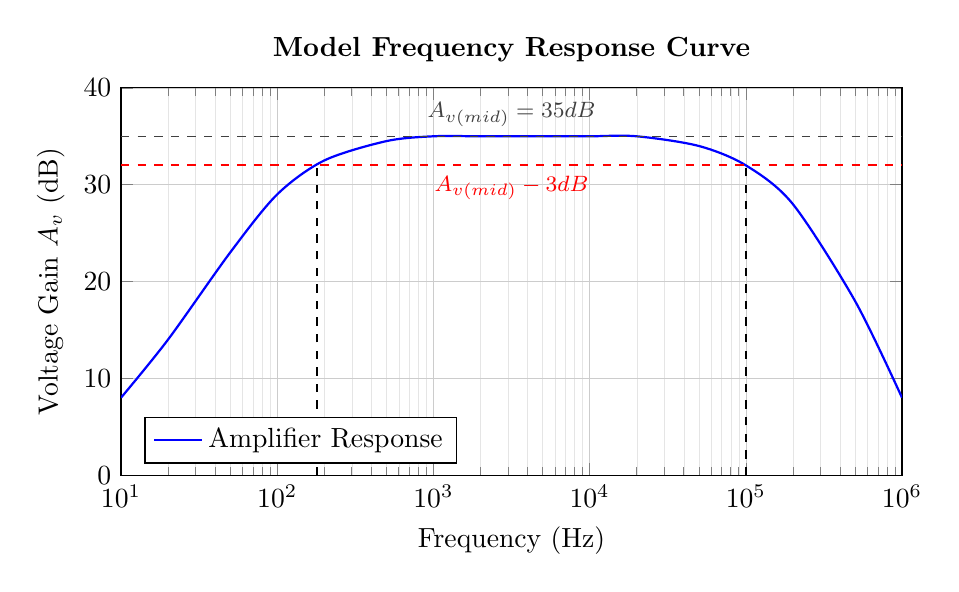
\begin{tikzpicture}
		\begin{semilogxaxis}[
			xlabel={Frequency (Hz)},
			ylabel={Voltage Gain $A_v$ (dB)},
			xmin=10, xmax=1000000,
			ymin=0, ymax=40,
			grid=both,
			grid style={line width=.1pt, draw=gray!20},
			major grid style={line width=.2pt, draw=gray!40},
			width=11.5cm, height=6.5cm,
			title={\textbf{Model Frequency Response Curve}},
			legend pos=south west
			]
			% Simulated smooth gain data
			\addplot[thick, color=blue, smooth] coordinates {
				(10, 8) (20, 14) (50, 23) (100, 29) (200, 32.5) (500, 34.5)
				(1000, 35) (2000, 35) (5000, 35) (10000, 35) (20000, 35)
				(50000, 34) (100000, 32) (200000, 28) (500000, 18) (1000000, 8)
			};
			\addlegendentry{Amplifier Response}
			
			% Midband level and -3dB line
			\draw[dashed, red, thick] (axis cs:10, 32) -- (axis cs:1000000, 32) node[below, pos=0.5] {\footnotesize $A_{v(mid)} - 3\text{ dB}$};
			\draw[dashed, darkgray, thin] (axis cs:10, 35) -- (axis cs:1000000, 35) node[above, pos=0.5] {\footnotesize $A_{v(mid)} = 35\text{ dB}$};
			
			% Cutoff markers
			\draw[dashed, black, thick] (axis cs:180, 0) -- (axis cs:180, 32);
			\draw[dashed, black, thick] (axis cs:100000, 0) -- (axis cs:100000, 32);
			
			% Labels for cutoff points
			\node[below] at (axis cs:100, 0) {$f_L$};
			\node[below] at (axis cs:100000, 0) {$f_H$};
		\end{semilogxaxis}
	\end{tikzpicture}
	\caption{Semi-logarithmic plot of the Expected Frequency Response}
	\label{fig:freq_response}
\end{figure}
\begin{figure}[h!]
	\centering
	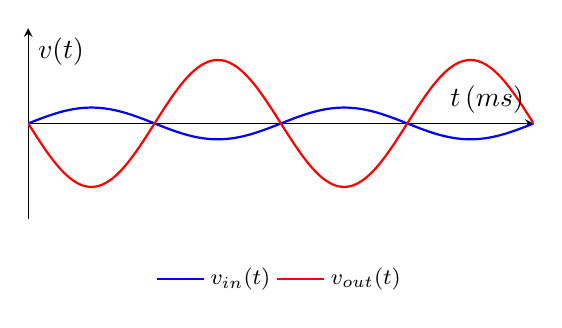
\begin{tikzpicture}
		\begin{axis}[
			width=8cm, height=4cm,
			xlabel={$t\, (ms)$}, ylabel={$v(t)$},
			axis lines=middle,
			%grid=major,
			ymin=-3, ymax=3,
			xtick=\empty, ytick=\empty,
			domain=0:2, samples=200,
			legend style={draw=none, font=\footnotesize, at={(0.5,-0.2)}, anchor=north, legend columns=2}
			]
			\addplot[blue, thick] {0.5*sin(360*x)};
			\addlegendentry{$v_{in}(t)$}
			\addplot[red, thick] {-2*sin(360*x)};
			\addlegendentry{$v_{out}(t)$}
		\end{axis}
	\end{tikzpicture}
	\caption{Expected input and (amplified, inverted) output waveforms in the mid-band region.}
	\label{fig:wave_ce}
\end{figure}

\section{Observations}
\subsection{DC Operating Point Parameters}
Record the measured static DC parameters in Table \ref{tab:dc_obs} and compare them with the calculated theoretical values.

\begin{table}[h!]
	\centering
	\begin{tabular}{lll}
		\toprule
		\textbf{Parameter} & \textbf{Theoretical Value} & \textbf{Measured Value} \\
		\midrule
		Base Voltage ($V_B$) &  & \\
		Emitter Voltage ($V_E$) & & \\
		Collector Voltage ($V_C$) &  & \\
		Collector-Emitter Voltage ($V_{CEQ}$) & &  \\
		Collector Current ($I_{CQ}$) &  &  \\
		\bottomrule
	\end{tabular}
	\caption{DC Operating Point Measurements}
	\label{tab:dc_obs}
\end{table}

\subsection{AC Frequency Response Data}
Record the input and output peak-to-peak voltages across the frequency range in Table \ref{tab:freq_response_obs}. Maintain $V_{in}$ constant.
\begin{table}[h!]
	\centering
	\begin{tabular}{@{}cccccc@{}}
		\toprule
		S. No. & Freq. $f$ (Hz) & $V_{in,pp}$ (V) & $V_{out,pp}$ (V) & $A_v = V_{out,pp}/V_{in,pp}$ & $A_v = 20\log_{10}(A_v)$ (dB) \\
		\midrule
		1& 10	&  &  &  &  \\
		2& 20	&  &  &  &  \\
		$\vdots$ & $\vdots$	&  &  &  &  \\
		$\vdots$&$\vdots$	&  &  &  &  \\
		$\vdots$&$\vdots$	&  &  &  &  \\
		& 500k	&  &  &  &  \\
		& 1M	&  &  &  &  \\
		\bottomrule
	\end{tabular}
	\caption{Frequency response data (add rows as needed to adequately capture the roll-off regions).}
	\label{tab:freq_response_obs}
\end{table}
%\subsection{Summary of Observations}
%Summarise the observations in Table~\ref{tab:summary}.
%\begin{table}[h!]
%	\centering
%	\begin{tabular}{@{}lccc@{}}
%		\toprule
%		Quantity & Design (theory) & LTspice (Pre-Lab) & Measured (hardware) \\
%		\midrule
%		$V_B$ (V) &  & -- &  \\
%		$V_E$ (V) &  & -- &  \\
%		$V_{CEQ}$ (V) &  & -- &  \\
%		$A_{v(mid)}(dB)$ &  &  &  \\
%		$f_L$ (Hz) &  &  &  \\
%		$f_H$ (Hz) &  &  &  \\
%		$BW$ (Hz) &  &  &  \\
%		\bottomrule
%	\end{tabular}
%	\caption{Summary: comparison of design, simulation, and hardware measurement.}
%	\label{tab:summary}
%\end{table}
%\clearpage
\newpage
\section{Result}

The RC-coupled CE amplifier was designed, assembled, and tested. The performance parameters of the single-stage RC-coupled BJT amplifier were experimentally measured and determined from the frequency response plot:
\begin{itemize}
	\item Measured Mid-Band Voltage Gain, $A_{v(mid)}$ = \rule{2cm}{0.15mm} (or \rule{2cm}{0.15mm} dB)
	\item Lower Cutoff Frequency, $f_L$ = \rule{2cm}{0.15mm} Hz
	\item Upper Cutoff Frequency, $f_H$ = \rule{2cm}{0.15mm} Hz
	\item Experimental Bandwidth ($BW = f_H - f_L$) = \rule{2cm}{0.15mm} Hz
\end{itemize}
The DC operating point was successfully verified, and the plotted frequency response reflects the expected drop in voltage gain at low and high frequencies.

\section{Questions}
\begin{enumerate}[label=Q\arabic*.]
	\item Why is voltage-divider bias preferred over fixed bias for BJT amplifier stages in terms of $Q$-point stability against $\beta$ variation?
	\item Explain, with reasoning, why the emitter bypass capacitor $C_E$ is essential for achieving high mid-band gain, and what happens to $A_{v(mid)}$ if $C_E$ is removed.
	\item Derive the expression for the lower cutoff frequency contributed by $C_{in}$ alone, treating all other capacitors as ideal AC shorts.
	\item What is the Miller effect, and how does it contribute to the reduction in gain at high frequencies in a CE amplifier?
	\item Why must the input signal amplitude be kept small during this experiment? What form of distortion would be observed if it were too large, and why?
	\item Compare the phase relationship between $v_{in}$ and $v_{out}$ in the CE amplifier with that of the RC network studied in Pre-Lab~1.
	%\item Why does the phase shift between the input and output voltages of a common-emitter amplifier equal exactly $180^\circ$?
	\item What would happen to the output signal if the input coupling capacitor $C_{in}$ developed an internal short circuit?
	\item How does the load resistance $R_L$ affect the mid-band voltage gain of the amplifier?
	\item Why is the common-emitter configuration the preferred choice for cascading multiple amplification stages compared to common-base or common-collector configurations?
	\item What is the function of the input coupling capacitor?
	\item Why is the emitter bypass capacitor used?
	\item Why does the output waveform undergo phase reversal in CE configuration?
	\item What is meant by midband gain?
	\item Define lower and upper cut-off frequencies.
	\item Why does gain decrease at low frequencies?
	\item Why does gain decrease at high frequencies?
	\item What is the significance of the \SI{-3}{dB} point?
	\item How is bandwidth related to the frequency response curve?
	\item Why should the transistor be properly biased before applying the input signal?
	\item What type of coupling is used between stages in an RC-coupled amplifier?
	\item How does changing $R_C$ affect the gain of the amplifier?
	\item Name one limitation of an RC-coupled amplifier.
\end{enumerate}
